\documentclass[french]{msereport}

\usepackage{minted}

\newcommand{\aws}{\brand{Amazon Web Services}}
\newcommand{\plex}{\brand{PLEX}}

\title{\plex\ in the Cloud with \aws}
\module{CLOUD}{Cloud Computing}
\author{Benjamen Burgy Jonathan Cornaz}

\begin{document}
	
	\section{Introduction}
		Le but de ce projet est de proposer un déploiement automatisé d’un serveur multimédia privé sur \aws.
		
		\plex\ (https://plex.tv) est une solution pour la gestion des fichiers multimédias. Il permet (entre autre) de facilement pouvoir naviguer dans sa bibliothèque multimédia et de directement regarder un film ou écouter de la musique. \plex\ peut être installé sur n’importe quelle machine et être lié à un support de stockage arbitraire, ce qui permet d’installer chez soi un serveur multimédia privé.
		
		Une des problématiques centrale à résoudre est que \plex\ ne propose pas de système de télé-versement des fichiers. Il a donc fallu développer une petite application web qui permet à l’utilisateur ayant déployé sont serveur multimédia de télé-verser ses fichiers.
	
	\section{Déploiement} 
		Le but est de déployer sur \aws\ trois entités distinctes, à savoir un emplacement pour le stockage de fichier (S3), un serveur de média \plex\ et une petite application web développé par nos soins. Le script doit automatiser un maximum les tâches à effectuer pour simplifier le déploiement à l’utilisateur.
		
		Il y a cependant des étapes que nous ne pouvons pas automatiser et que l’utilisateur doit effectuer lui-même :
		\begin{itemize}
			\item Créer un compte \aws\ (s’il n’en a pas déjà un)
			\item Créer et télé-charger une paire de clé pour la connexion SSH
			\item Créer fichier de config YAML
			\item Installer les dépendances
			\begin{itemize}
				\item Python et PIP
				\item \code{pip install -r requirements.txt}
			\end{itemize}
			\item Exécuter le script de déploiement (\code{python deploy.py \textless config\_file\textgreater})
		\end{itemize}
		
		Le fichier de config permet à l'utilisateur de choisir quel IP public utiliser (elastic ip) pour chaque service, ainsi que le nom de l'emplacement de stockage S3. De plus il permet de renseigner les infromations de connexion nécessaires pour effectuer des opération sur \aws.
	
		\begin{minted}[
			gobble=3,
				frame=lines,
				fontsize=\footnotesize,
				label=Structure du fichier de configuration (YAML)
			]{xml}
			access:
				id: <aws-access-id>
				key: <aws-access-key>
				ssh_key: <path-to-the-ssh-key>
			
			elastic_ips:
				plex: <publicip-for-the-media-server>
				file_uploader: <publicip-for-the-web-server>
			
			bucket_name: <S3-storage-bucket-name>
		\end{minted}

		Le script de déploiement charge le fichier de configuration, se connect à \aws\ et acommence par créer un espace de stockage ou de simplement y accéder si celui-ci existe déjà. Il démarre ensuite des machines EC2 (une pour \plex\ et une pour le serveur web), configurer les machines pour pointer vers l’espace de stockage et démarre leur services respectifs.
		
		Au début, nous aurions voulu utiliser la technologie docker, et plus particulièrement le service de conteneur EC2 d'amazon. Ce choix était principalement motivé par la volonté d'essayer cette technologie. Dans la pratique cela ne s'est révélé pas pertinent, puisque notre projet n'est pas orienté pour le développement et la maintenance d'une application mufti-tiers. Nous somme principalement orienté déploiement de machine dans sur \aws. Pour cette raison nous avons finalement utilisé des machines EC2 et un emplacement de stockage S3 pour notre déploiement.
		
	\section{S3 Storage }
		Le but est d’avoir une zone de stockage centrale des fichiers télé-versés par l’application web et utilisable par le serveur de média \plex. Nous avons donc créée une instance pour un emplacement de stockage S3 (bucket). Cela a été fait via un script afin de pouvoir proposer ce déploiement à des tiers qui n’aurait alors qu’à spécifier le nom de l’emplacement de stockage qu’ils désirent.
		
		Une fois un espace de stockage instancié, il convient de se poser la question de la façon d’y accéder à ces données. En l'occurrence, nous ne pouvions pas modifier \plex\ et avons donc choisi de pouvoir “monter” cet espace de stockage comme un système de fichier dans les machines.
		
		Pour y arriver plusieurs solutions existent et nous avons évalué la possibilité d'utiliser \brand{s3fs} (\brand{fuse}), \brand{s3backer} (qui se basent sur le précédent) et \brand{s3ql}. Le problème avec \brand{fuse}, est qu’il est nécessaire d’obtenir l’intégralité d’un fichier avant de pouvoir l’utiliser. Comme il est question ici d’un serveur de média, cela implique des fichiers volumineux, et il n’est pas envisageable de forcer l’utilisateur à attendre que son film soit complètement télé-chargé par le serveur de média avant qu’il puisse le regarder. C’est pourquoi nous avons opté pour \brand{s3ql}. Ce dernier crée un système de fichier qui lui est propre et découpe les fichiers en petits blocs (10mo par défaut).
	
	\section{Serveur PLEX}		
		Nous avons créé une machine et y avons installé \plex\ ainsi que \brand{s3ql}. Nous avons fait une image de cette machine et l’avons rendu publique ce qui nous permet de proposé un script qui instancie une machine depuis cette image, sans avoir besoin de diffuser des informations sensibles concernant notre compte \aws.
		
		Comme il n'est pas possible que plusieurs machines montent simultanément le même "bucket" viar s3ql, il faut également que le serveur \plex\ partage sont dossier sur le réseau via NFS. Comme ce partage doit être restreint uniquement au serveur web, ceci ne peut se faire qu'au déploiement. Les outils nécessaires à ce partages ont été installé sur l'image utilisée et le script de dépoloiement ajoute le partage spécifié dès que l'instance à été crée et qu'il connait l'adresse ip privée de du serveur web.
		
		Le script de déploiement se charge donc d’instancier une nouvelle machine sur la base de cette image, d’y envoyer les informations de connexion à l’emplacement de stockage (access-id et access-key), de monter le stockage dans un dossier (/mnt/s3), de partager ce stockage avec le serveur web (via NFS) et démarrer le service \plex.
	
	\section{Application Web}
		Nous avons développé une petite application dans le but de gérer le stockage des médias de Plex à travers le web. L’application permet des opérations simples dans sa première version comme l’ajout de répertoires et fichiers et leurs suppression. Elle supporte le télé-chargement sur le S3 storage de fichiers de grandes tailles.
		
		L’application utilise le concept de Single Page Application en utilisant les librairies \brand{AngularJS}, \brand{Bootstrap} pour la partie client et \brand{Flask} pour la partie serveur en python.
		
		Le serveur peut être configuré par le biais d’un fichier settings.yml à la racine du serveur. L’installation de l’application web se fait facilement avec les commandes suivantes:
		
		\code{pip install -r requirements.txt --upgrade \&\& bower install \&\& python index.py}
		
		\begin{figure}[h]
			\label{webserver}
			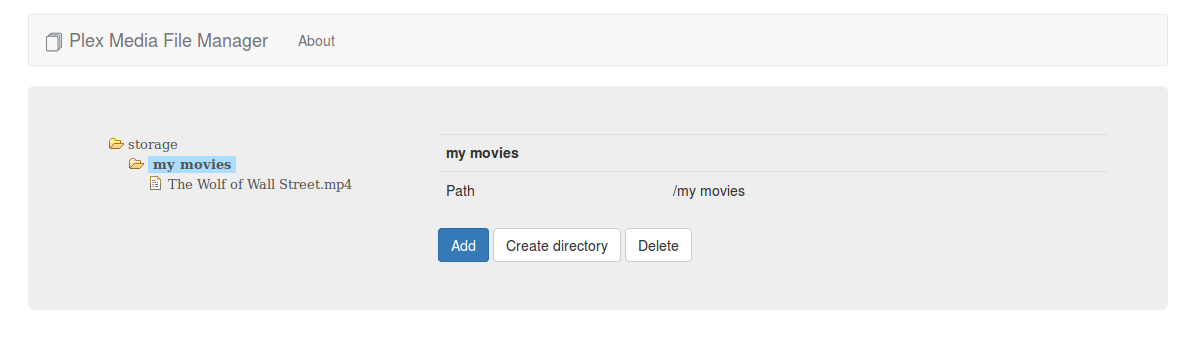
\includegraphics[width=\textwidth]{screen_webserver.png}
			\caption{Application web}
		\end{figure}
	
		Il est a noter que cette application web nécessite python 3.5 pour pouvoir tourner correctement. Dans les machines EC2 il a donc fallu entreprendre des actions d'administration pour réussir à obtenir l'environnement python adéquat.
	
	\section{Conclusion}
		Nous avons pu développer et déployé l'embryon d’une application qui pourrait séduire de nombreux clients désirant un stockage privé sur une infrastructure solide et performante tel que le propose \aws.
		
		Le déploiement utilise les dernières technologies et nous avons pu rendre facile l'instalation autant la partie \plex\ que de la partie web à travers quelques lignes de commande utilisant Python comme langage de programmation pour l’automatisation.
	
	\appendixsection
	
		\listoffigures
		
		\subsection{Sources}
			Les sources sont livrées avec le présent rapport et peuvent être obtenues sur notre repository github: \url{https://github.com/slimaku/hesso.cloud.plex}
	
\end{document}
